\section{Results, Statistical Benchmark, and Aerodynamic Validation}
\label{sec:results}

\subsection{Equal-Budget Search Benchmark Outcomes}
\label{sec:budget_results}
Table~\ref{tab:budget} and Fig.~\ref{fig:equal_budget} report every strategy of Section~\ref{sec:budget_protocol} after 287 evaluations beyond the shared pool, whose best feasible design reaches \NvPool\,km. Table~\ref{tab:tests} gives the \NvNfamily\ headline comparisons, which Fig.~\ref{fig:forest} shows with their intervals.

\begin{table}[htbp]
\centering\small
\caption{Equal-budget search performance on the shared 9,800-design pool; strategy names as in Section~\ref{sec:budget_protocol}. Range: mean running best after 100 evaluations (pool included), mean $\pm$ standard deviation of the best feasible range after 287 evaluations, and its extremes over runs. Evaluations: share that is feasible over the whole run (valid) and over the first 60 evaluations (valid$_{60}$), and share spent on designs that violate the washout ordering (fail $g_8$). Beating the pool: number of runs that exceed the best pool design and the median number of evaluations needed. One AL run and one AL-R run stopped early by exhaustion and are included with the value they reached.}
\label{tab:budget}
\begin{tabular*}{\linewidth}{@{\extracolsep{\fill}}lrrrrrrrrr@{}}
\toprule
 & & \multicolumn{3}{c}{Best feasible range (km)} & \multicolumn{3}{c}{Share of evaluations (\%)} & \multicolumn{2}{c}{Beating the pool} \\
\cmidrule(lr){3-5}\cmidrule(lr){6-8}\cmidrule(l){9-10}
Strategy & Runs & at 100 & at 287 & min to max & valid & valid$_{60}$ & fail $g_8$ & runs & evals \\
\midrule
TuRBO & 20 & 382.9 & 396.8 $\pm$ 4.4 & 385.3 to 403.0 & 82 & 80 & 0 & 20/20 & 2 \\
AL-R & 20 & 378.8 & 391.5 $\pm$ 6.6 & 367.9 to 399.5 & 64 & 24 & 0 & 20/20 & 31 \\
AL & 11 & 374.1 & 385.0 $\pm$ 10.4 & 368.9 to 397.4 & 59 & 14 & 17 & 11/11 & 43 \\
adapt10 & 20 & 372.9 & 386.1 $\pm$ 6.3 & 369.2 to 393.2 & 68 & 69 & 0 & 20/20 & 34 \\
local10 & 10 & 358.8 & 365.2 $\pm$ 4.7 & 358.5 to 373.1 & 64 & 60 & 0 & 10/10 & 36 \\
local5 & 10 & 359.3 & 364.2 $\pm$ 6.6 & 351.9 to 373.2 & 81 & 80 & 0 & 9/10 & 31 \\
LHS & 10 & 352.9 & 298.3 $\pm$ 27.2 & 260.2 to 337.3 & 28 & 30 & 0 & 0/10 & n/a \\
Uniform & 10 & 352.9 & 307.6 $\pm$ 30.5 & 264.2 to 353.3 & 28 & 26 & 0 & 1/10 & 147 \\
\midrule
Pool only & n/a & n/a & 352.9 & n/a & 28 & n/a & 0 & n/a & n/a \\
\bottomrule
\end{tabular*}

\end{table}

\begin{figure}[htbp]
\centering
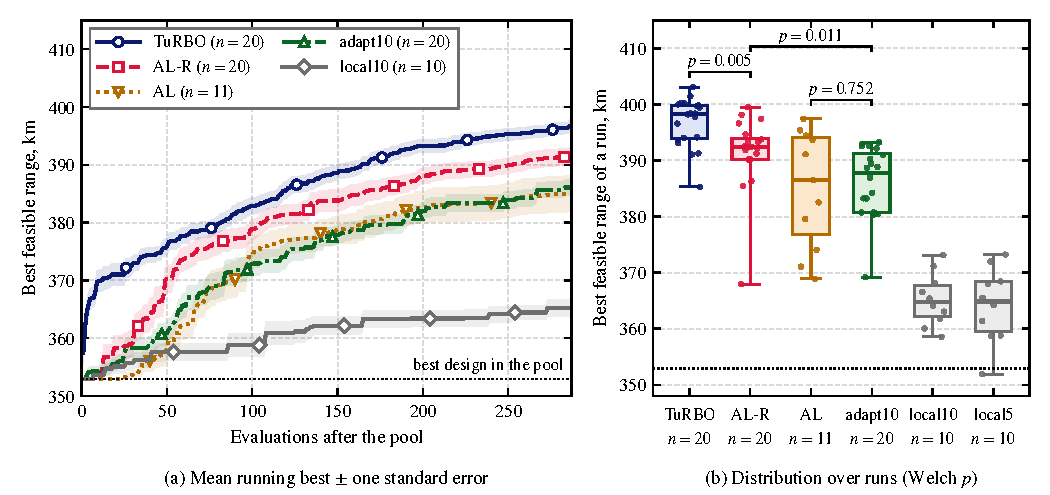
\includegraphics[width=\linewidth]{figures/fig_equal_budget.pdf}
\caption{Equal-budget benchmark. (a) Mean running best feasible range, pool included, against the number of evaluations beyond the pool for the five leading strategies; the bands are $\pm$ one standard error over seeds and the dotted line is the best design in the pool. (b) Best feasible range of every run (dots) for the six strategies that improve on the pool; the box spans the quartiles, the line is the median and the whiskers reach the extremes. Brackets give two-sided Welch $p$-values, not corrected for multiplicity (Table~\ref{tab:tests} gives the corrected values). Fresh Latin hypercube and uniform sampling end below the pool best and are listed in Table~\ref{tab:budget} only.}
\label{fig:equal_budget}
\end{figure}

\begin{table}[htbp]
\centering\small
\caption{Headline comparisons of best feasible range after 287 evaluations. Welch and Mann--Whitney tests are two-sided; Holm correction is applied over the \NvNfamily\ rows; M--W is the Mann--Whitney test; the interval is a percentile bootstrap on the difference of means; $P(A{>}B)$ is the share of run pairs in which $A$ ends above $B$.}
\label{tab:tests}
\begin{tabular*}{\linewidth}{@{\extracolsep{\fill}}lcrrrrrcr@{}}
\toprule
 & & \multicolumn{2}{c}{Difference} & \multicolumn{3}{c}{Two-sided $p$} & & \\
\cmidrule(lr){3-4}\cmidrule(lr){5-7}
$A$ minus $B$ & $n_A$, $n_B$ & km & \% & Welch & Holm & M--W & 95\% CI (km) & $P(A{>}B)$ \\
\midrule
TuRBO $-$ AL-R & 20, 20 & $+5.3$ & $+1.4$ & 0.005 & 0.020 & 0.001 & $[2.2,\ 8.8]$ & 0.80 \\
AL-R $-$ AL & 20, 11 & $+6.5$ & $+1.7$ & 0.079 & 0.159 & 0.180 & $[0.1,\ 12.9]$ & 0.65 \\
AL-R $-$ adapt10 & 20, 20 & $+5.4$ & $+1.4$ & 0.011 & 0.033 & 0.003 & $[1.4,\ 9.2]$ & 0.78 \\
TuRBO $-$ adapt10 & 20, 20 & $+10.7$ & $+2.8$ & $<$0.001 & $<$0.001 & $<$0.001 & $[7.5,\ 14.1]$ & 0.94 \\
AL $-$ adapt10 & 11, 20 & ${-}1.1$ & ${-}0.3$ & 0.752 & 0.752 & 0.918 & $[-7.6,\ 5.1]$ & 0.51 \\
adapt10 $-$ local10 & 20, 10 & $+20.9$ & $+5.7$ & $<$0.001 & $<$0.001 & $<$0.001 & $[16.9,\ 24.6]$ & 0.99 \\
AL $-$ local10 & 11, 10 & $+19.8$ & $+5.4$ & $<$0.001 & $<$0.001 & $<$0.001 & $[13.2,\ 26.1]$ & 0.96 \\
\bottomrule
\end{tabular*}

\end{table}

Four results follow.

\textbf{TuRBO is the strongest strategy.} It reaches $\NvMeanTurbo \pm \NvSdTurbo$\,km over \NvNTurbo\ seeds, \NvGainPctTurbo\% above the pool best, with the highest feasible fraction (\NvValidTurbo\%) and an improvement on the pool within the first few evaluations of every run. It exceeds the adaptive local search by \NvDTurbovAdapt\,km (Holm $p \NvHTurbovAdapt$) and the published active-learning loop by \NvDTurbovAL\,km (Welch $p \NvPTurbovAL$, bootstrap 95\% interval $\NvCITurbovAL$\,km).

\textbf{Active learning with the washout repair is second.} AL-R reaches $\NvMeanALR \pm \NvSdALR$\,km over \NvNALR\ seeds. TuRBO leads it by \NvDTurbovALR\,km (\NvPctTurbovALR\%; Welch $p \NvPTurbovALR$, Mann--Whitney $p \NvUTurbovALR$, Holm $p \NvHTurbovALR$; interval $\NvCITurbovALR$\,km), a lead that remains significant after Holm correction. The size of the lead depends on one run: AL-R seed 16 exhausted its candidate list after 83 evaluations at \NvMinALR\,km. Without that run AL-R averages $\NvMeanALRc \pm \NvSdALRc$\,km and the gap to TuRBO is \NvDTurbovALRc\,km (Welch $p \NvPTurbovALRc$, interval $\NvCITurbovALRc$\,km). Early exhaustion occurred in one of \NvNALR\ AL-R runs and one of \NvNAL\ AL runs and in no run of any other strategy; it is a reliability cost of the surrogate loop and is kept in the headline numbers. AL-R exceeds the adaptive local search by \NvDALRvAdapt\,km (Holm $p \NvHALRvAdapt$).

\textbf{The published active-learning loop is not better than a surrogate-free adaptive local search.} AL reaches $\NvMeanAL \pm \NvSdAL$\,km and adapt10 $\NvMeanAdapt \pm \NvSdAdapt$\,km; the difference is $\NvDsALvAdapt$\,km (Welch $p \NvPALvAdapt$, interval $\NvCIALvAdapt$\,km). The loop spent \NvWashAL\% of its evaluations on designs that fail the washout ordering $g_8$, which no other strategy could propose. Removing that asymmetry raises the mean by \NvDALRvAL\,km (Welch $p \NvPALRvAL$, Holm $p \NvHALRvAL$) and, on the ten matched seeds analyzed in Section~\ref{sec:feas_ablation}, by \NvDALRtenvALrep\,km (Welch $p \NvPALRtenvALrep$). The surrogate therefore earns a measurable margin over random proposals around the same parent set only once the loop is prevented from proposing designs that a one-line repair would fix.

\textbf{Moving the search center matters more than the surrogate.} Static local search around the 20 best pool designs reaches $\NvMeanLocTen \pm \NvSdLocTen$\,km, and letting the parent set follow new discoveries adds \NvDAdaptvLocTen\,km (Holm $p \NvHAdaptvLocTen$). Measured against the gain of TuRBO over the pool best, static local search recovers \NvShareLocTen\%, adaptive local search \NvShareAdapt\%, published active learning \NvShareAL\%, and AL-R \NvShareALR\%. Fresh Latin hypercube and uniform sampling do not improve on the pool in a 287-evaluation allocation except in one uniform run.

\textbf{The ordering does not depend on where the budget is cut.} Table~\ref{tab:anytime} repeats the comparison at 50, 100, 150 and 200 evaluations. TuRBO has the highest mean and AL-R the second highest at every budget; the lead of TuRBO over AL-R is between \NlAnyTRlo\ and \NlAnyTRhi\,km and reaches the 5\% level (uncorrected) from \NlAnyTRsigFrom\ evaluations onward, and AL-R exceeds the adaptive local search at every budget (Welch $p \le \NlAnyRApmax$). The published loop and the adaptive local search remain within a few kilometers of each other throughout.

\textbf{Doubling the budget narrows the gaps but keeps the ordering.} TuRBO and the adaptive local search (seeds 0 to 9) and AL-R (seeds 0 to 4) were continued from 287 to \NlBudget\ evaluations (Table~\ref{tab:long}). TuRBO reaches $\NlTurboCMean \pm \NlTurboCSd$\,km, the adaptive local search $\NlAdaptCMean \pm \NlAdaptCSd$\,km and AL-R $\NlALRCMean \pm \NlALRCSd$\,km. The second 287 evaluations add \NlTurboGain\,km for TuRBO and \NlAdaptGain\,km for the adaptive local search, so on these ten seeds the lead of TuRBO over the surrogate-free search falls from \NlTvAAD\ to \NlTvACD\,km (Welch $p = \NlTvACP$), while its lead over AL-R on the five shared seeds is \NlTvRCD\,km ($p = \NlTvRCP$). No run of any strategy exceeds \NlAllMax\,km within the original bounds. The strategies therefore approach a common ceiling, which Section~\ref{sec:bound_prices} attributes to the bounds, and the advantage of a model is largest when evaluations are scarce.

\begin{table}[htbp]
\centering\small
\caption{Best feasible range (km, mean $\pm$ standard deviation, pool included) when the runs are continued to twice the budget, and differences between strategies with two-sided Welch $p$-values (not corrected for multiplicity).}
\label{tab:long}
% generated by make_numbers_long.py; do not edit
\begin{tabular*}{\linewidth}{@{\extracolsep{\fill}}lrrr@{}}
\toprule
Evaluations beyond the pool & 287 & 400 & 574 \\
\midrule
TuRBO ($n=10$) & 396.3 $\pm$ 5.3 & 399.2 $\pm$ 4.5 & 400.9 $\pm$ 3.8 \\
AL-R ($n=5$) & 394.8 $\pm$ 3.2 & 395.7 $\pm$ 3.5 & 397.0 $\pm$ 4.1 \\
adapt10 ($n=10$) & 386.1 $\pm$ 7.7 & 391.9 $\pm$ 7.6 & 395.4 $\pm$ 5.7 \\
\midrule
TuRBO minus adapt10, km (Welch $p$) & $+10.2$ (0.003) & $+7.3$ (0.020) & $+5.5$ (0.022) \\
TuRBO minus AL-R, seeds 0 to 4, km (Welch $p$) & $+3.3$ (0.201) & $+4.5$ (0.066) & $+5.8$ (0.031) \\
AL-R minus adapt10, seeds 0 to 4, km (Welch $p$) & $+11.6$ (0.058) & $+5.9$ (0.273) & $+4.3$ (0.286) \\
\bottomrule
\end{tabular*}

\end{table}

Table~\ref{tab:asrun} lists the corrected baselines beside their first implementations. For TuRBO the correction of the energy basis changes the mean by $\NvPairedTurboD$\,km (paired over the same \NvPairedTurboN\ seeds, $p \NvPairedTurboP$), because every trust region starts from a new evaluation within its first batches and then compares new evaluations with each other. For the adaptive local search it raises the mean by \NvDAdaptvAdaptOld\,km (Welch $p \NvPAdaptvAdaptOld$): the first implementation kept too many early evaluations in the parent set. The correction therefore strengthens the surrogate-free baseline that the active-learning loop is compared with.

\subsection{Sensitivity to the Size of the Initial Pool}
\label{sec:pool_size}
The benchmark above shares one pool of 9{,}800 designs, which is $97\%$ of all evaluations. To test whether the conclusions depend on that pool, TuRBO, the adaptive local search and AL-R were rerun from random subsamples of 288, 1{,}000 and 3{,}000 pool designs, with the same 287 further evaluations. The subsample is drawn with a seed tied to the run seed, so the three strategies start from the same designs in runs with the same seed. The outcome of a run is the best feasible range among its subsample and its own evaluations (Table~\ref{tab:pool}, Fig.~\ref{fig:pool_size}).

\begin{table}[htbp]
\centering\small
\caption{Best feasible range (km, mean $\pm$ standard deviation) after 287 evaluations from pools of different size. TuRBO and adapt10: seeds 0 to 9; AL-R: seeds 0 to 4. The last row repeats the runs of the main benchmark with the same seeds. ``Pool best'' is the mean best design of the subsamples. The row marked independent uses ten separately generated 1{,}000-design pools, one per seed, in place of subsamples.}
\label{tab:pool}
\resizebox{\linewidth}{!}{%
% generated by make_numbers_pool.py; do not edit
\begin{tabular}{@{}rrrrrrrr@{}}
\toprule
Pool size & Total evaluations & Pool best (km) & TuRBO (km) & adapt10 (km) & AL-R (km) & TuRBO minus adapt10 (km) & Welch $p$ \\
\midrule
288 & 575 & 295.8 & 388.0 $\pm$ 9.0 & 374.5 $\pm$ 8.4 & 386.1 $\pm$ 5.4 & $+13.5$ & 0.003 \\
1{,}000 & 1{,}287 & 330.3 & 394.2 $\pm$ 5.8 & 377.4 $\pm$ 8.7 & 392.4 $\pm$ 7.1 & $+16.9$ & <0.001 \\
3{,}000 & 3{,}287 & 338.5 & 393.5 $\pm$ 9.1 & 382.4 $\pm$ 8.4 & 390.1 $\pm$ 5.3 & $+11.0$ & 0.011 \\
9{,}800 & 10{,}087 & 352.9 & 396.3 $\pm$ 5.3 & 386.1 $\pm$ 7.7 & 394.8 $\pm$ 3.2 & $+10.2$ & 0.003 \\
\midrule
1{,}000, independent & 1{,}287 & 313.1 & 388.3 $\pm$ 10.0 & 379.8 $\pm$ 9.7 & not run & $+8.6$ & 0.068 \\
\bottomrule
\end{tabular}

}
\end{table}

\begin{figure}[htbp]
\centering
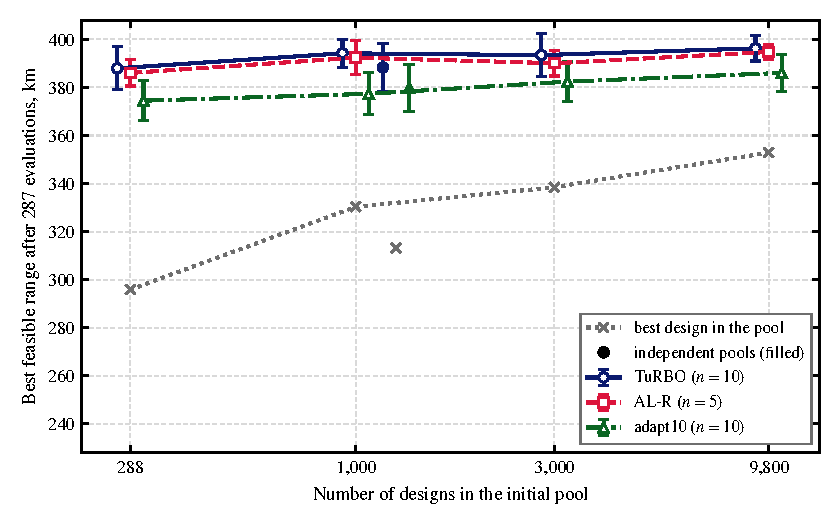
\includegraphics[width=0.8\linewidth]{figures/fig_pool_size.pdf}
\caption{Best feasible range after 287 evaluations as a function of the size of the initial pool (mean and standard deviation over seeds; the three strategies are offset horizontally for clarity). The dotted line is the mean best design in the pool before the search. Filled symbols at 1{,}000 designs are the runs from independent pools.}
\label{fig:pool_size}
\end{figure}

\textbf{A subsample one tenth the size of the pool costs the model-based strategies little.} From 1{,}000 pool designs TuRBO reaches \NpTurboBMean\,km, which is \NpTurboLossB\,km below its result from the full pool (Welch $p = \NpTurboLossBP$, bootstrap 95\% CI $\NpTurboLossBCI$\,km); from 3{,}000 designs the difference is \NpTurboLossC\,km ($p = \NpTurboLossCP$). Only the smallest pool costs a measurable amount: \NpTurboLossA\,km, or $\NpTurboLossAPct\%$ ($p = \NpTurboLossAP$). AL-R behaves in the same way on five seeds (\NpALRLossB\,km at 1{,}000 designs, $p = \NpALRLossBP$; \NpALRLossA\,km at 288, $p = \NpALRLossAP$). These non-significant differences are not evidence of equivalence, and the interval for TuRBO at 1{,}000 designs still allows a loss of several kilometers. They do show that most of the pool is not needed to reach the neighborhood of the best designs. This agrees with benchmark studies of unconstrained Bayesian optimization on test functions, which found small initial designs preferable~\cite{bossek2020initial,leriche2021revisiting}; the present result extends that observation to a constrained aircraft problem in which most of the sample is infeasible.

\textbf{A pool no larger than the search budget is enough to exceed the full pool.} With 288 initial designs and 287 further evaluations, \NpEvalsA\ in total, all \NpTurboABeatFull\ TuRBO runs and all \NpAdaptABeatFull\ adaptive-local runs end above the best of the 9{,}800 pool designs (\NpFullPoolBest\,km); the worst TuRBO run reaches \NpTurboAMin\,km. For comparison, the best design of a 288-design space-filling subsample averages \NpPoolABest\,km. Sequential search of any of the three kinds is therefore far more efficient than the space-filling sample on this problem, with about \NpEvalRatio\ times fewer evaluations for a longer range.

\textbf{The ordering of the strategies does not depend on the pool.} TuRBO is ahead of the adaptive local search at every pool size, by \NpTvAAD, \NpTvABD, \NpTvACD\ and \NpTvAFD\,km from the smallest pool to the full one ($p \le \NpTvAMaxP$ in each case), and TuRBO and AL-R are not distinguishable at any size on the five shared seeds ($p \ge \NpTvRMinP$). The surrogate-free search depends on the pool more than TuRBO does: it loses \NpAdaptLossB\,km at 1{,}000 designs ($p = \NpAdaptLossBP$) and \NpAdaptLossA\,km at 288 ($p = \NpAdaptLossAP$), because its parents are pool designs until better ones are found. The advantage of the model-based strategies over the surrogate-free control is therefore not produced by the large pool, and it is at least as large when the pool is small.

\textbf{Independent pools give a less favorable but consistent picture.} The subsamples above are drawn from the one pool and can inherit its best designs. As a check, ten fresh Latin hypercube pools of 1{,}000 designs were generated and evaluated, one for each seed, and TuRBO and the adaptive local search were run from them (last row of Table~\ref{tab:pool}, filled symbols in Fig.~\ref{fig:pool_size}). The best design of these pools averages \NpIndPoolBest\,km, against \NpPoolBBest\,km for the subsamples of the same size. TuRBO reaches $\NpIndTurboMean \pm \NpIndTurboSd$\,km, which is \NpIndTurboVsSubAbs\,km below its result on the subsamples (Welch $p = \NpIndTurboVsSubP$) and \NpIndTurboVsFull\,km below its result from the full pool ($p = \NpIndTurboVsFullP$); the adaptive local search reaches $\NpIndAdaptMean \pm \NpIndAdaptSd$\,km. TuRBO leads by \NpIndTvAD\,km (bootstrap 95\% CI $\NpIndTvACI$\,km, Welch $p = \NpIndTvAP$), the same direction as in every other row of the table but not significant at the 5\% level with ten runs. All \NpIndTurboBeatFull\ TuRBO runs and all \NpIndAdaptBeatFull\ adaptive-local runs again exceed the best of the full pool, with \NpIndEvals\ evaluations in total. Taken together, reducing the pool from 9{,}800 to 1{,}000 designs costs TuRBO between \NpTurboLossB\ and \NpIndTurboVsFull\,km ($\NpTurboLossBPct$ to $\NpIndTurboVsFullPct\%$), depending on whether the small pool happens to contain good designs. The means are also not monotone in the pool size (TuRBO at 3{,}000 against 1{,}000 designs), which shows the size of the seed-to-seed noise at ten runs.

\subsection{Role of the Classifier Weight and of the Washout Repair}
\label{sec:feas_ablation}
Table~\ref{tab:factorial} crosses the two ingredients of the active-learning acquisition that concern feasibility: the classifier weight $w(P_{\mathrm{feas}})$ (sigmoid, hard gate at $P_{\mathrm{feas}} \ge 0.5$, or absent) and the washout repair (sorting the four twist variables before evaluation). Each cell uses seeds 0 to 9.

\begin{table}[htbp]
\centering\small
\caption{Feasibility handling in the active-learning acquisition, ten seeds per row (TuRBO: 20, as in Table~\ref{tab:budget}), and the effect of adding the sigmoid weight to TuRBO (TuRBO+w). ``Sigmoid'', ``hard gate'' and ``none'' are the forms of the classifier weight and ``+R'' is the washout repair. Columns as in Table~\ref{tab:budget}.}
\label{tab:factorial}
\begin{tabular*}{\linewidth}{@{\extracolsep{\fill}}lrrrrrrrrr@{}}
\toprule
 & & \multicolumn{3}{c}{Best feasible range (km)} & \multicolumn{3}{c}{Share of evaluations (\%)} & \multicolumn{2}{c}{Beating the pool} \\
\cmidrule(lr){3-5}\cmidrule(lr){6-8}\cmidrule(l){9-10}
Strategy & Runs & at 100 & at 287 & min to max & valid & valid$_{60}$ & fail $g_8$ & runs & evals \\
\midrule
AL, sigmoid & 10 & 376.1 & 385.5 $\pm$ 10.8 & 368.9 to 397.4 & 60 & 14 & 17 & 10/10 & 44 \\
AL, sigmoid + R & 10 & 379.8 & 394.0 $\pm$ 4.1 & 386.3 to 399.5 & 65 & 26 & 0 & 10/10 & 32 \\
AL, none & 10 & n/a & none feasible & n/a & 0 & 0 & 100 & 0/10 & n/a \\
AL, none + R & 10 & n/a & none feasible & n/a & 0 & 0 & 0 & 0/10 & n/a \\
AL, hard gate & 10 & 352.9 & 394.0 $\pm$ 4.2 & 383.6 to 399.5 & 10 & 0 & 64 & 10/10 & 192 \\
TuRBO & 20 & 382.9 & 396.8 $\pm$ 4.4 & 385.3 to 403.0 & 82 & 80 & 0 & 20/20 & 2 \\
TuRBO+w & 10 & 383.9 & 397.5 $\pm$ 2.8 & 394.0 to 403.0 & 92 & 92 & 0 & 10/10 & 2 \\
\bottomrule
\end{tabular*}

\end{table}

\begin{figure}[htbp]
\centering
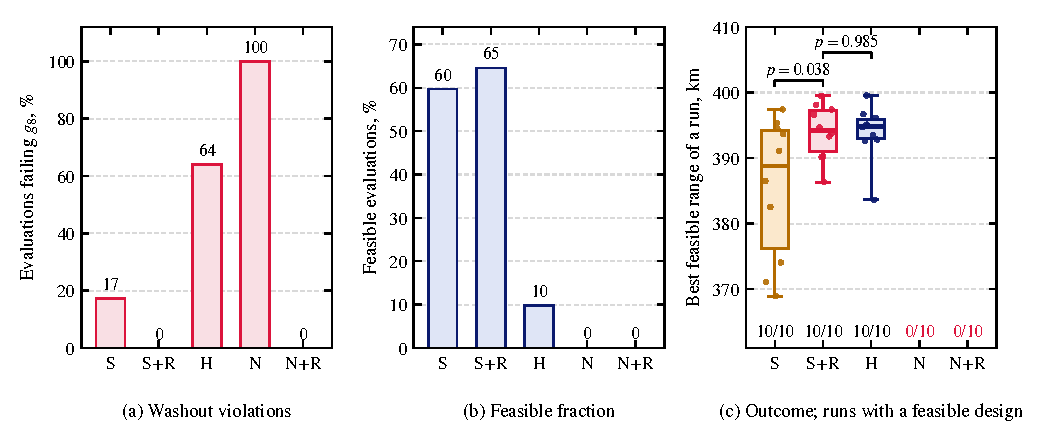
\includegraphics[width=\linewidth]{figures/fig_repair.pdf}
\caption{Feasibility handling in the active-learning loop (seeds 0 to 9). S: sigmoid weight; H: hard gate; N: no weight; +R: with the washout repair. (a) Share of evaluations that violate the washout ordering $g_8$ (\%; the repair makes it zero). (b) Share of feasible evaluations (\%). (c) Best feasible range of every run (dots) with quartiles, median and extremes; brackets give two-sided Welch $p$-values and the figures above the axis the number of runs that found a feasible design.}
\label{fig:repair}
\end{figure}

\textbf{Without a classifier weight the loop finds no feasible design.} This holds in all ten runs without the repair and in all ten runs with it. The regression surrogates are fitted on feasible designs only, so they carry no information about the constraint boundary, and the optimizer of the acquisition settles in a corner of the box (short center body, minimum blend chord, maximum battery mass) where the predicted range is high and the bay volume constraint $g_6$ is violated. The classifier is therefore a necessary component of this loop and not an optional refinement.

\textbf{The form of the weight is secondary.} A hard gate reaches $\NvMeanALhard \pm \NvSdALhard$\,km without the repair, against $\NvMeanALRten \pm \NvSdALRten$\,km for the sigmoid weight with the repair (no difference at the resolution of the table, Welch $p \NvPALhardvALRten$). The gate reaches this value late: only \NvValidALhard\% of its evaluations are feasible and its first improvement on the pool comes after a median of 192 evaluations, so its result at smaller budgets is worse than that of the sigmoid weight.

\textbf{The repair accounts for the gap between the published loop and AL-R.} With the sigmoid weight, sorting the twist variables raises the mean from $\NvMeanALrep \pm \NvSdALrep$ to $\NvMeanALRten \pm \NvSdALRten$\,km (\NvDALRtenvALrep\,km, Welch $p \NvPALRtenvALrep$, Mann--Whitney $p \NvUALRtenvALrep$, interval $\NvCIALRtenvALrep$\,km) and removes the low tail of the distribution (Fig.~\ref{fig:repair}). The evidence for this effect is moderate, not strong: the Mann--Whitney test does not reach the 5\% level, and with all available seeds the Holm-corrected value in Table~\ref{tab:tests} is $p \NvHALRvAL$.

\textbf{The weight does not help TuRBO.} Applying the same sigmoid weight to the Thompson samples of TuRBO changes the mean by $\NvDsTurboFeasFixvTurbo$\,km (Welch $p \NvPTurboFeasFixvTurbo$, bootstrap 95\% CI $\NvCITurboFeasFixvTurbo$\,km) while raising the feasible fraction from \NvValidTurbo\% to \NvValidTurboFeasFix\%. The same experiment with the first TuRBO implementation gave $\NvDsTurboFeasvTurboOld$\,km ($p \NvPTurboFeasvTurboOld$; Table~\ref{tab:asrun}), so neither version shows a gain in the mean. A trust region centered on a feasible design already keeps most candidates feasible, so the classifier adds little there. The weight is a requirement of a global acquisition built on feasible-only surrogates, not a general improvement to constrained search.

\subsection{Surrogate Distribution Shift and Extrapolation Performance}
\label{sec:distribution_shift}
The loop samples where the surrogate predicts high range, so the designs it proposes are not distributed like the pool on which the surrogate was trained. Two tests quantify the effect on the ensemble: (i) training on the pool and testing on the 157 feasible designs proposed by the original campaign, and (ii) a deliberately harsh extrapolation test, training on designs with $R < 250\,\mathrm{km}$ and testing on those with $R \ge 250\,\mathrm{km}$.

Table~\ref{tab:shift} and Fig.~\ref{fig:surrogate_parity} show a clear loss of accuracy. On the designs proposed by the loop the coefficient of determination for range falls from $0.997$ in cross-validation to $R^2 = \NshiftRtwo$, with a mean absolute error of $\NshiftMae\,\mathrm{km}$ that is almost entirely a bias ($\NshiftBias\,\mathrm{km}$): the ensemble underpredicts the range of the best designs. The rank correlation over all test designs remains high ($\rho = 0.95$), and $78\%$ of the test points lie within one ensemble standard deviation. Within the best tenth of the test designs, however, the rank correlation for range is close to zero ($\rho = -0.05$; $-0.02$ in the extrapolation test), and in the extrapolation test $R^2$ falls to $0.35$. The ensemble thus separates good designs from poor ones but does not order the best designs among themselves. This is consistent with the benchmark result that a search guided by this ensemble gains little over a local search that uses no surrogate (Section~\ref{sec:budget_results}).

\subsection{Cross-Solver Consistency with AeroBuildup}
\label{sec:aerobuildup_consistency}
\label{sec:validation}
To check that the ranking produced by the pipeline does not depend on its drag model, the pipeline was compared with AeroBuildup on $\NxN$ designs: the six best and six randomly chosen feasible designs of each of the first three seeds of the clamp and no-clamp searches of Section~\ref{sec:loft}, so that half of the sample comes from the top of the ranking. AeroBuildup is evaluated at the cruise lift coefficient of the pipeline.

As shown in Fig.~\ref{fig:aerobuildup_polar} and Fig.~\ref{fig:fidelity_suite}(a), the two solvers rank the designs alike: the Spearman correlation of $L/D$ is $\rho = \NxRho$ over the whole set and $\rho = \NxRhoTop$ among the 36 top designs. The absolute values differ considerably. AeroBuildup gives a higher $L/D$ than the pipeline on every design, with a median ratio of $\NxRatioMed$ (5th to 95th percentile $\NxRatioLo$ to $\NxRatioHi$). The difference comes mainly from profile drag: AeroBuildup uses NeuralFoil section polars with predicted transition, which give about two thirds of the pipeline's strip estimate (Supplementary Section~\ref{sec:neuralfoil_audit}). The pipeline is therefore pessimistic in absolute range relative to these models, and the absolute ranges in this paper should be read as estimates of a low-order model whose drag level has not been validated by experiment.

\paragraph{Panel refinement, section drag and Euler solutions} Three further checks are reported in the Supplementary Material and summarized in Fig.~\ref{fig:fidelity_suite}. Refining the lattice from 672 to 3{,}584 panels changes $L/D$ of the good designs by $0.6$ to $1.5\%$ and the static margin by less than $0.009$; only poor designs with closely spaced sections are sensitive to the finest grids, which become ill-conditioned (Supplementary Section~\ref{sec:grid_convergence}). NeuralFoil section polars give $0.60$ to $0.65$ times the strip estimate of profile drag with free transition and about $1.18$ times with forced transition, with little variation between designs, so the ranking is unaffected while the absolute range depends on how much laminar flow the airframe achieves (Supplementary Section~\ref{sec:neuralfoil_audit}). Euler solutions of five designs reproduce the lattice lift within $4\%$ for the three designs with a cruise $C_L$ above $0.2$, but give a static margin higher than the lattice value on every design, by a factor of $1.14$ to $1.28$; the best design of the original campaign has $SM = \NcfdChampSM$ in the Euler solution, above the $0.25$ limit (Supplementary Section~\ref{sec:cfd_validation}). Because the lattice underpredicts the margin, it is not conservative with respect to the upper limit, which motivates the calibration that follows.

\begin{figure*}[htbp]
\centering
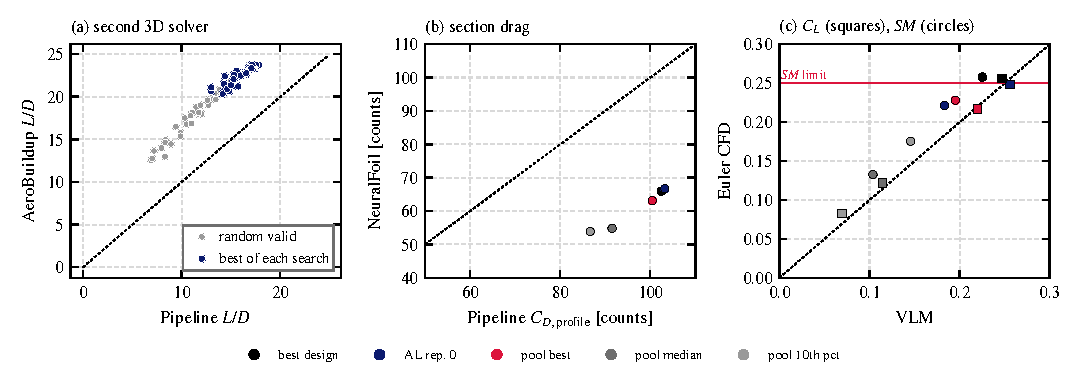
\includegraphics[width=\linewidth]{figures/fig_fidelity.pdf}
\caption{Multi-fidelity aerodynamic verification suite across computational tiers. (a) Cross-solver consistency between the baseline VLM pipeline and AeroBuildup across $n=72$ designs (Spearman $\rho = 0.98$ overall, $\rho = 0.91$ among the 36 top designs; median ratio $1.46$). (b) Viscous profile drag comparison between empirical strip theory and NeuralFoil ($e^N$ transition) across five representative configurations, with a ratio between $0.60$ and $0.65$. (c) 3D compressible Euler CFD using SU2 ($\sim 1.2 \times 10^5$ nodes) versus VLM predictions for lift coefficient $C_L$ (squares) and longitudinal static margin $SM$ (circles). The $C_L$ ratio lies between $0.97$ and $1.19$ and the Euler static margin is $1.14$ to $1.28$ times the lattice value. The best design of the original campaign reaches $SM = 0.258$ in the Euler solution, above the $0.25$ limit, whereas the best design of active-learning replication 0 has $SM = 0.221$.}
\label{fig:fidelity_suite}
\end{figure*}

\subsection{Calibrating the Static-Margin Constraint Against Euler CFD}
\label{sec:sm_calibration}
Five designs cannot define a correction for the static margin. The Euler analysis was therefore extended to \NcalNnew\ further designs, giving \NcalN\ in total: the best valid design of each of five search arms (TuRBO, active learning, adaptive local search, local search at $\pm 10\%$ and at $\pm 5\%$), and ten designs whose lattice margin lies near $0.05, 0.072, \ldots, 0.25$ (the valid design closest to each target among those with range at or above the pool median). Each case uses the setup of Supplementary Section~\ref{sec:cfd_validation} ($h = 7\,\mathrm{mm}$, $M = 0.11$, two angles of attack $2^\circ$ apart), and the Euler margin is $SM_{\mathrm{Euler}} = -\Delta C_{m}/\Delta C_{L}$ between them.

\begin{figure}[htbp]
\centering
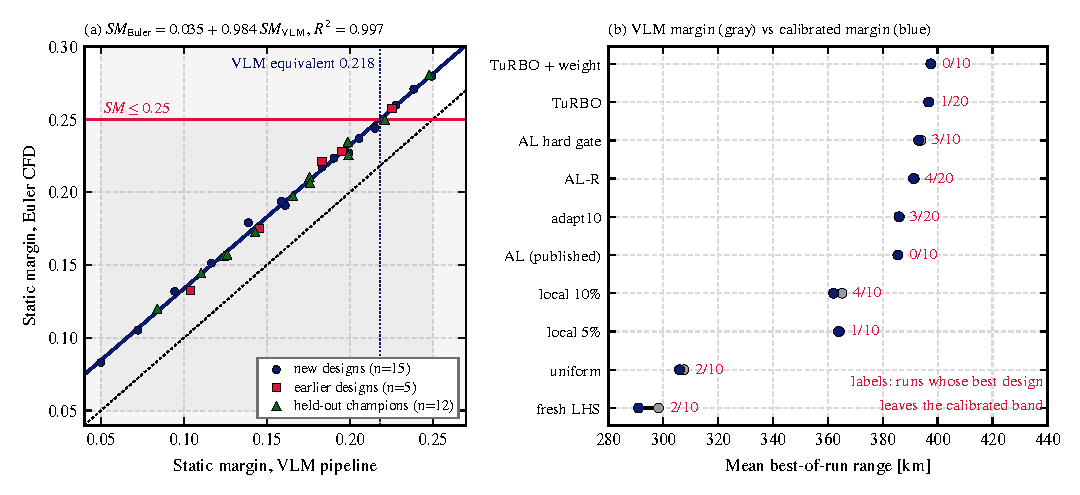
\includegraphics[width=\linewidth]{figures/fig_sm_calibration.pdf}
\caption{Calibration of the lattice static margin against Euler CFD. (a) Euler margin versus lattice margin for the \NcalN\ designs of the fit (circles and squares) with the least-squares line (blue), and for the \NoosN\ held-out run champions (triangles); the horizontal line is the $0.25$ cap and the dotted vertical line its lattice equivalent. (b) Mean best-of-run range of each search arm with the original lattice constraint (gray) and with the calibrated constraint applied after the fact (blue); the labels give the number of runs whose best design falls outside the calibrated band $0.05 \le SM \le 0.25$.}
\label{fig:sm_calibration}
\end{figure}

The relation is close to a constant shift (Fig.~\ref{fig:sm_calibration}a). A least-squares fit gives $SM_{\mathrm{Euler}} = \NcalA + \NcalB\,SM_{\mathrm{VLM}}$ with $R^2 = \NcalRsq$ and a residual standard deviation of \NcalSd; the 95\% bootstrap intervals are \NcalAci\ for the intercept and \NcalBci\ for the slope, so the slope is consistent with one and the offset with a constant of about \NcalA. The earlier ratio of $1.14\times$ to $1.28\times$ was therefore the same additive offset seen at different margins. The $C_L$ ratio between Euler and the lattice has a median of \NcalCLmed\ (range \NcalCLlo\ to \NcalCLhi) and does not show a trend. The offset moves the cap: $SM_{\mathrm{Euler}} \le 0.25$ corresponds to $SM_{\mathrm{VLM}} \le \NcalCapEquiv$, so a design that the optimizer treats as having a margin of $0.24$ has a margin near $0.27$ in Euler CFD. The lower cap of $0.05$ corresponds to a lattice value of \NcalFloorEquiv\ and is not active. A $5\,\mathrm{mm}$ surface mesh for the active-learning champion ($\NcalAlHfiveNodes\times 10^3$ nodes) changes its Euler margin from \NcalAlHsevenSM\ to \NcalAlHfiveSM\ ($\NcalAlHdelta\%$), far below the offset.

\paragraph{Out-of-sample check of the calibration} The fit above was made first and then frozen. Afterwards, Euler solutions were computed with the same setup for \NoosN\ further designs that played no part in it: the best design of six TuRBO runs, three AL-R runs and three adaptive-local runs of the corrected benchmark (Table~\ref{tab:oos}). Their lattice margins span \NoosVlmLo\ to \NoosVlmHi. The frozen line predicts the Euler margin of these designs with a root-mean-square error of \NoosRmse, a mean error of \NoosBias\ and a largest error of \NoosMax, which is the same size as the residual standard deviation of the fit (\NoosFitSd). The calibration therefore holds for the designs that the searches actually converge to, and not only for the designs it was fitted on. The check also bears on the cap. The calibration places \NoosPredOver\ of the \NoosN\ designs above $0.25$; the Euler solution confirms \NoosEulerOver\ (\NoosEulerHi) and puts the other at \NoosNearCap, which is on the cap to within the error of the fit. A decision closer to the cap than about \NoosMax\ therefore cannot be made from the calibrated lattice value alone.

\begin{table}[htbp]
\centering\small
\caption{Out-of-sample check of the static-margin calibration on \NoosN\ run champions that were not used in the fit. The prediction is $\NcalA + \NcalB\,SM_{\mathrm{VLM}}$ with the coefficients of Section~\ref{sec:sm_calibration} unchanged.}
\label{tab:oos}
% generated by b13_oos_validate.py; do not edit
\begin{tabular}{llrrrr}
\toprule
Strategy & Seed & Lattice $\mathrm{SM}$ & Predicted Euler $\mathrm{SM}$ & Euler $\mathrm{SM}$ & Error \\
\midrule
AL-R & 10 & 0.084 & 0.118 & 0.120 & $+0.002$ \\
TuRBO & 2 & 0.110 & 0.144 & 0.144 & $+0.000$ \\
TuRBO & 3 & 0.124 & 0.158 & 0.156 & $-0.001$ \\
TuRBO & 5 & 0.126 & 0.160 & 0.157 & $-0.002$ \\
AL-R & 11 & 0.143 & 0.176 & 0.173 & $-0.003$ \\
TuRBO & 0 & 0.166 & 0.198 & 0.198 & $-0.001$ \\
adapt10 & 12 & 0.176 & 0.208 & 0.210 & $+0.002$ \\
TuRBO & 4 & 0.176 & 0.209 & 0.206 & $-0.002$ \\
AL-R & 12 & 0.199 & 0.231 & 0.234 & $+0.004$ \\
adapt10 & 10 & 0.199 & 0.231 & 0.225 & $-0.006$ \\
TuRBO & 1 & 0.221 & 0.253 & 0.250 & $-0.003$ \\
adapt10 & 11 & 0.248 & 0.279 & 0.281 & $+0.001$ \\
\midrule
\multicolumn{5}{l}{Root-mean-square error} & 0.003 \\
\multicolumn{5}{l}{Largest absolute error} & 0.006 \\
\bottomrule
\end{tabular}

\end{table}

Table~\ref{tab:sm_rerank} applies the fitted correction after the fact to every run: the best-of-run range is recomputed over the designs that satisfy $0.05 \le a + b\,SM_{\mathrm{VLM}} \le 0.25$. No search was repeated, and only designs that the original run had accepted can be recovered, so the calibrated feasible set is a subset of the original one. The effect on the mean best range is small for the adaptive strategies, at most \NcalLossAlHard\,km, and the ranking of the arms does not change. What changes is feasibility. The best design lies outside the calibrated band in \NcalOutLocTen\ of \NcalOutNLocTen\ static local-search ($\pm 10\%$) runs, \NcalOutAlHard\ of \NcalOutNAlHard\ runs of active learning with a hard gate, \NcalOutAlR\ of \NcalOutNAlR\ AL-R runs, \NcalOutAdapt\ of \NcalOutNAdapt\ adaptive-local runs and \NcalOutTurbo\ of \NcalOutNTurbo\ TuRBO runs, and in none of the \NcalOutNAlSoft\ runs of the published loop. The effect is therefore not confined to one kind of strategy: any search that converges toward the upper limit of the margin can end slightly beyond the calibrated limit. In each such run another design within the band is almost as good, which is why the loss in range is small. This agrees with the CFD result for the original campaign champion ($SM_{\mathrm{Euler}} = 0.258$). Euler CFD is itself an inviscid model, so the calibration maps one low-order model onto a better one and does not establish the true margin; wind-tunnel or flight data would be needed for that.

\subsection{Range Cost of Each Bound}
\label{sec:bound_prices}
Section~\ref{sec:bound_sensitivity} shows that relaxing four bounds together raises the range, but not which bound matters. To measure that, TuRBO was rerun on the same pool and budget with exactly one bound widened by $10\%$ of that variable's range, five seeds per bound: the lower taper-ratio bound ($0.55 \to 0.525$), the upper winglet-twist bound ($0 \to +1^\circ$), the upper battery-mass bound ($3.5 \to 3.7\,\mathrm{kg}$), and the lower cruise-speed bound ($36.1 \to 33.6\,\mathrm{m/s}$). The speed bound is the $130\,\mathrm{km/h}$ mission requirement, so that run measures what the requirement costs, not an engineering limit. The lower bound of $c_{\mathrm{blend}}$ could not be tested because the geometry code clips $c_{\mathrm{blend}}$ to at least $0.25\,\mathrm{m}$ regardless of the bound. The reference is the same TuRBO implementation on the original bounds ($n = 10$, \NbpRefMean\,km $\pm$ \NbpRefSd\,km). These runs use the corrected TuRBO implementation; the same experiment with the first implementation is retained in the data archive and gave the same pattern, with a measurable price for the battery-mass bound only.

\begin{table}[htbp]
\centering\small
\caption{Range gained by widening a single bound by $10\%$ of its range (TuRBO, 287 evaluations after the pool, five seeds per bound), against TuRBO on the original bounds. The confidence interval is a bootstrap interval on the difference of means (20{,}000 resamples), and $p$ is a two-sided Welch test. The last column is the share of runs whose best design lies within $2\%$ of the variable's range of the new limit. The cruise-speed bound is the mission requirement.}
\label{tab:bound_prices}
\begin{tabular*}{\linewidth}{@{\extracolsep{\fill}}llrrrcrr@{}}
\toprule
 & & & & \multicolumn{3}{c}{Gain over the original bounds} & \\
\cmidrule(lr){5-7}
Bound & Change & Runs & Best (km) & km & 95\% CI (km) & Welch $p$ & At new bound \\
\midrule
None & original bounds & 10 & 396.3 $\pm$ 5.3 & n/a & n/a & n/a & n/a \\
Taper ratio, lower & $0.55 \to 0.525$ & 5 & 398.7 $\pm$ 7.3 & $+2.4$ & $[-4.5,\ 8.3]$ & 0.530 & 60\% \\
Winglet twist, upper & $0 \to +1^\circ$ & 5 & 395.7 $\pm$ 4.3 & $-0.6$ & $[-5.1,\ 4.0]$ & 0.831 & 0\% \\
Battery mass, upper & $3.5 \to 3.7$\,kg & 5 & 417.3 $\pm$ 3.0 & $+21.0$ & $[17.2,\ 25.0]$ & $<$0.001 & 100\% \\
Cruise speed, lower & $36.1 \to 33.6$\,m/s & 5 & 395.8 $\pm$ 3.5 & $-0.5$ & $[-4.5,\ 3.9]$ & 0.831 & 0\% \\
\bottomrule
\end{tabular*}

\end{table}

Only the battery-mass bound has a measurable price (Table~\ref{tab:bound_prices}, Fig.~\ref{fig:bound_robust}a): raising it by $0.2\,\mathrm{kg}$ gained \textbf{$\NbpBmassGain$\,km} ($+\NbpBmassGainPct\%$, bootstrap 95\% CI $\NbpBmassCI$\,km, $p \NbpBmassP$), and every run ended at the new limit. That is close to proportional, since the extra mass is \NbpBmassMassPct\% of the bound and the range gain is \NbpBmassGainPct\%, as expected when the energy carried sets the range. The other three bounds gave $\NbpTaperGain$\,km (taper, $p = \NbpTaperP$), $\NbpWtwistGain$\,km (winglet twist, $p = \NbpWtwistP$) and $\NbpSpeedGain$\,km (speed, $p = \NbpSpeedP$), each indistinguishable from zero with five runs; their confidence intervals ($\NbpTaperCI$, $\NbpWtwistCI$ and $\NbpSpeedCI$\,km) leave room for gains of a few kilometers, so small effects cannot be excluded. With the speed bound lowered, \NbpSpeedAtBound\% of the runs ended near the new limit, so the search did not use the extra room. The optimum is therefore limited mainly by how much energy the airframe may carry, and a search in the nominal box cannot trade that against the other variables.

\begin{figure}[htbp]
\centering
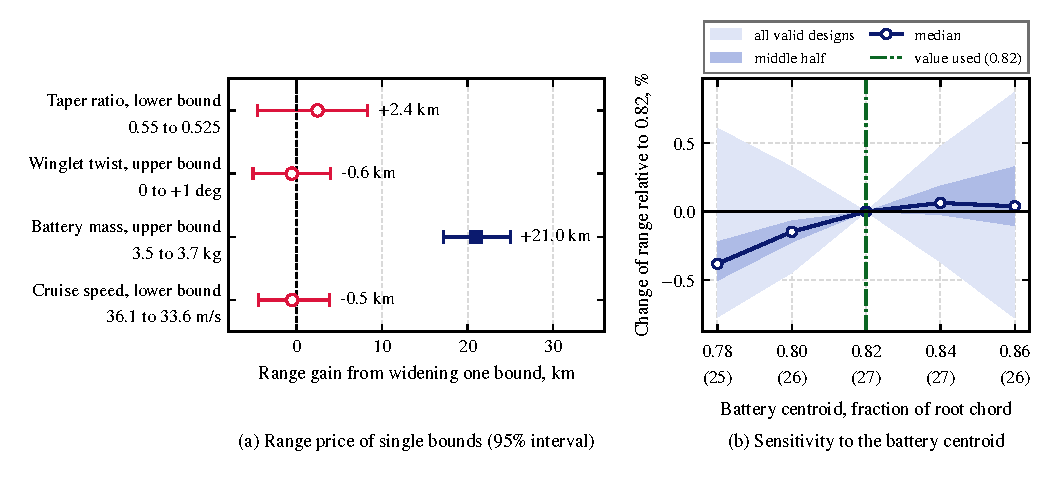
\includegraphics[width=\linewidth]{figures/fig_bound_robust.pdf}
\caption{(a) Range gained by widening each bound by 10\% of its range: difference of means against TuRBO on the original bounds with bootstrap 95\% intervals; the filled square is significant (Welch $p < 0.05$). (b) Change of calm-air range when the battery centroid is moved between 0.78 and 0.86 of the root chord, relative to the default 0.82, over the best designs of all search arms: median, middle half and full spread of the designs that remain valid, whose number is given in parentheses.}
\label{fig:bound_robust}
\end{figure}

\subsection{Robustness to the Battery Centroid and Battery Mass}
\label{sec:robustness}
The optimization fixes the battery centroid at $0.82\,c_{r}$ (Section~\ref{sec:dynamic_balance}). To check how much the conclusions depend on that value, \NrbN\ designs (the twenty best valid designs found by any arm, the best design of each arm and the original campaign champion, without duplicates) were reevaluated with the full pipeline at centroid positions from $0.78$ to $0.86\,c_{r}$ and with the battery mass changed by $\pm 5\%$. Moving the centroid by $\pm 0.04\,c_{r}$ changes the range by at most \NrbBandLossMax\% for any design that stays valid (Fig.~\ref{fig:bound_robust}b), and \NrbBandValid\ of the \NrbN\ designs stay valid over the whole interval. The best design that survives every perturbation is \NrbAllBest\ with \NrbAllBestRange\,km, which loses \NrbAllBestMfiveLoss\% of its range when the battery mass is reduced by $5\%$ and gains \NrbAllBestPfiveGain\% when it is increased; reducing the mass costs about \NrbMfiveLossMean\% of range on average, in line with the energy carried. The $+5\%$ case makes \NrbPfiveInvalid\ of the \NrbN\ designs invalid, and every one of these failures comes from the evaluator's check that rejects designs whose span efficiency factor exceeds one (values between $1.000$ and $1.006$). The best designs thus lie at the edge of a region the evaluator considers non-physical, which is a further active limit that is not among the box bounds and is consistent with reading the optima as boundary-limited. Only \NrbAllValid\ of the \NrbN\ designs are valid in all five centroid positions and both mass changes.

\subsection{Characteristics of the Audited Designs}
\label{sec:champion_characteristics}
Table~\ref{tab:best} lists the characteristics of the best design of the original campaign and of the best design of active-learning replication 0, the two designs for which Euler solutions and all audits are available. Neither is the best design found in the benchmark (Table~\ref{tab:budget}).

\paragraph{What the best designs of the benchmark have in common} Figure~\ref{fig:champions} shows the best design of each of the \NwinN\ runs of TuRBO, AL-R and the adaptive local search. Two variables are at a bound in nearly every run: the battery mass is within $3\%$ of its range from the upper bound in $\NwinBmassAt\%$ of the runs and the cruise speed within $3\%$ of the lower bound in $\NwinSpeedAt\%$. The blend chord and the taper ratio are at their lower bounds in $\NwinCblendAt\%$ and $\NwinTaperAt\%$ of the runs. The other ten variables are not determined by the search: across runs their standard deviation is $\NwinFreeSdLo\%$ to $\NwinFreeSdHi\%$ of the allowed range. The \NwinTopN\ runs that end within \NwinTopBand\,km of the best run have $L/D$ between \NwinTopLDlo\ and \NwinTopLDhi\ with inner sweeps from $\NwinTopSwInLo^\circ$ to $\NwinTopSwInHi^\circ$, outer sweeps from $\NwinTopSwOutLo^\circ$ to $\NwinTopSwOutHi^\circ$ and lattice static margins from \NwinTopSMlo\ to \NwinTopSMhi. The range is therefore set by the energy carried, the cruise speed and a small wing area, and it is nearly flat in sweep, twist distribution and winglet geometry at this fidelity. The strategies also settle in different parts of this flat region: the best TuRBO designs have a longer root chord and a blend station further inboard than the best AL-R designs (mean $c_r$ of \NwinTurboCr\ against \NwinAlrCr\,m and mean $y_b$ of \NwinTurboYb\ against \NwinAlrYb\,m, Mann--Whitney $p \NwinCrP$ and $p \NwinYbP$), at ranges that differ by about one percent. A conceptual study of this kind can thus report the active bounds and the attainable range with some confidence, but it does not identify a unique planform.

\begin{figure}[htbp]
\centering
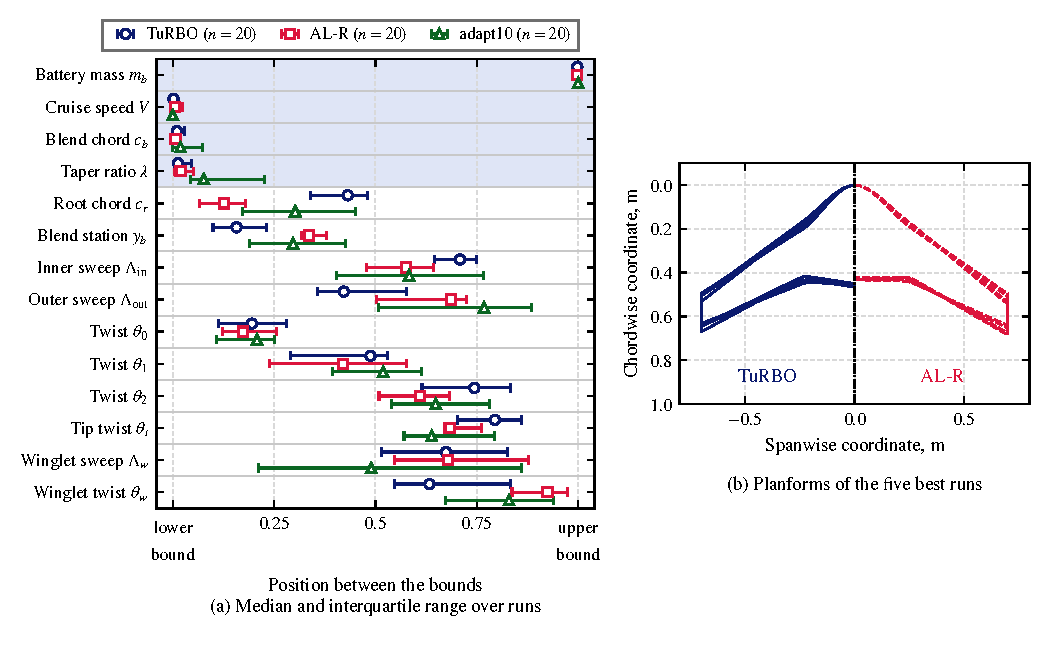
\includegraphics[width=\linewidth]{figures/fig_champions.pdf}
\caption{Best design of every run of TuRBO, AL-R and the adaptive local search. (a) Position of each design variable between its bounds: median and interquartile range over the runs of each strategy; the four shaded variables are those that end at a bound. (b) Planforms, without winglets, of the five best TuRBO runs (left, solid) and the five best AL-R runs (right, dashed).}
\label{fig:champions}
\end{figure}

The best design of the original campaign has an aspect ratio of $\NchAR$ and a reference area of $S_{\mathrm{ref}} = \NchSref\,\mathrm{m^2}$. At a cruise speed of $V = \NchV\,\mathrm{m/s}$ ($\NchVkmh\,\mathrm{km/h}$) the pipeline gives $L/D = \NchLD$, a calm-air range of $R = \NchampRange\,\mathrm{km}$, a lattice static margin of $SM = \NchSMpct\%$ and a cruise pitching moment of $C_m = \NchCm$. Its center of gravity lies at $42\%$ of the mean aerodynamic chord, slightly aft of the $15$ to $40\%$ window that the evaluator penalizes softly. The best designs of the benchmark runs differ from it mainly in using almost the full battery-mass allowance ($3.45$ to $3.50\,\mathrm{kg}$) close to the lowest permitted cruise speed.
